\chapter{Revisão de Literatura}

% \section{Planejamento e estimativas em metodologias ágeis}

  As metodologias ágeis se baseiam nos valores ágeis publicados no Manifesto Ágil
  (BECK, 2001 \textit{apud} \citeonline{cohn06}), que são:
  
  \begin{itemize}
   \item Indivíduos e interações entre eles mais que processos e ferramentas;
   \item Software em funcionamento mais que documentação abrangente;
   \item Colaboração com o cliente mais que negociação de contratos;
   \item Responder a mudanças mais que seguir um plano.
  \end{itemize}
  
 Seguir uma metodologia ágil em um projeto, também implica em uma abordagem ágil nas estimativas e planejamento, seguindo 
 os valores supracitados \cite{cohn06}. Conceitos importantes são necessários para entender o planejamento e estimativas
 num projeto ágil, como: iteração e \textit{sprints}, \textit{story points}, \textit{velocity}, entre outros.
 Esses conceitos serão devidamente aprofundados nas próximas seções.
 
\section{Tempo de trabalho: \textit{Sprints}}
 
 Times ágeis trabalham em iterações, que são um período de tempo fixo (\textit{time-boxed}) curto, de não mais que
 um mês de duração \cite{cohn06} \cite{scrum13}. O \textit{Scrum}, um \textit{framework} estrutural ágil, 
 traz o conceito de \textit{Sprint} para o processo de desenvolvimento, que nada mais é que um \textit{container} 
 temporal fixo para outros eventos do \textit{Scrum} \cite{scrum13}. Numa \textit{Sprint} é produzido um incremento 
 do \textit{software}, com base no que foi estabelecido como escopo daquela \textit{Sprint}. Como uma \textit{Sprint} possui
 a duração fixa, mesmo que uma funcionalidade não tenha sido completada nesta \textit{Sprint}, a mesma é encerrada no prazo
 que foi determinado \cite{cohn06}.
 
 De acordo com \citeonline{scrum13}, a 
 \textit{sprint} é composta pela reunião de planejamento da \textit{sprint}, reuniões diárias, trabalho de desenvolvimento,
 revisão da \textit{sprint} e retrospectiva da \textit{sprint}. Os esforços de estimativas se concentram na reunião de
 planejamento da \textit{sprint}, onde são estimadas as histórias de usuários. No começo de cada \textit{sprint}, o time 
 incorpora todo o conhecimento obtido com a \textit{sprint} passada para adaptar e ajustar o planejamento da próxima
 \textit{sprint} \cite{cohn06}.
 
\section{Estimativas com \textit{Story Points}}

 Em um projeto ágil 
 que utiliza histórias de usuário, pode-se estimar o tamanho de uma história em \textit{story points}.
 \textit{Story points} representam o tamanho geral de uma história, envolvendo o esforço necessário, a complexidade e os
 riscos inerentes para desenvolver a história \cite{cohn06}. O número atribuído à história como seu tamanho não é relevante,
 o que importa é o valor relativo entre as histórias, que é obtido por comparação entre elas \cite{cohn06}.
 
  \subsection{\textit{Velocity}}
  
    Numa abordagem ágil, a estimativa do tamanho é separada da estimativa da duração \cite{cohn06}.
    Com o tamanho estimado, é preciso de outro conceito para se calcular a duração, o \textit{velocity}.
    O \textit{velocity} mede a taxa de progresso do time, dizendo quantos pontos o time é capaz de desenvolver
    numa \textit{sprint}, podendo ser calculado como a soma dos pontos concluídos durante a iteração \cite{cohn06}.
    A melhor forma de se estabelecer o \textit{velocity} para um time é executando uma ou duas iterações e estimar o
    \textit{velocity} a partir do \textit{velocity} observado \cite{cohn06}.
 
  \subsection{Estimando a duração}
    
    Com o tamanho do \textit{software} e o \textit{velocity} do time de desenvolvimento conhecido, fica fácil estimar
    um prazo para o projeto, dividindo o tamanho pelo \textit{velocity}, obtendo assim a quantidade de \textit{sprints}
    necessárias, e multiplicando pelo tamanho da \textit{sprint} \cite{cohn06}.
    
    Utilizando uma abordagem por \textit{story points} em um projeto, separa-se completamente a estimativa do esforço
    necessário da estimativa da duração do projeto, permitindo que ambos sejam estimados independentemente. A estimativa de
    duração do projeto passa a ser derivada da estimativa de esforço \cite{cohn06}.
 
  \subsection{Escala das estimativas}
  \label{estimation_scales}
    
      Utilizar uma única ordem de magnitude gera estimativas melhores (Miranda 2001; Saaty 1996 \textit{apud} \cite{cohn06}).
      De acordo com \citeonline{cohn06}, uma escala de estimativa bastante utilizada e que se mostra bastante eficaz é a
      sequência \textit{Fibonnaci}, que consiste em pontuar as histórias utilizando algum número da 
      sequência 1, 2, 3, 5, 8, 13, [...]. É importante estabelecer um valor máximo para a sequência para manter o intervalo
      conhecido e não demasiado grande.
    
  \subsection{\textit{Planning Poker}}
  
    O \textit{Planning Poker} é uma técnica utilizada para estimativas ágeis que envolve as três técnicas de estimativa
    mais comuns (opnião do especialista, analogia e desagregação), gerando estimativas rápidas e confiáveis \cite{cohn06}.
    
    Todos os desenvolvedores participam do \textit{Planning Poker}, que se inicia com a entrega das cartas que contém os 
    valores válidos para as histórias na escala definida (vide a sub-seção \ref{estimation_scales}).
    Uma história é selecionada e é lida sua descrição pelo moderador
    do jogo (usualmente o \textit{Product Owner}, que não participa das estimativas) para que então os jogadores possam 
    avaliar a história e pontuá-la. Se houver divergências entre as pontuações, é iniciado um debate para que seja definida
    a pontuação final da história. Uma nova rodada é jogada novamente para a mesma história caso os participantes não
    entrem em um consenso \cite{grenning02}.
    
    O objetivo é fazer com o que os participantes convirjam para uma estimativa que será utilizada como pontuação da
    história, lembrando que a proposta do \textit{Planning Poker} não é gerar uma estimativa acurada que perdure por
    todo o ciclo de desenvolvimento, pois para atingir tal estimativa seria gasto um esforço 
    desnecessário \cite{cohn06} \cite{grenning02}.
    
    \citeonline{cohn06} diz que existe uma acurácia máxima para uma estimativa
    em relação ao esforço necessário para realizá-la, como ilustra a Figura \ref{fig:effort_accuracy}.
    Portanto, não é preciso um debate demorado e detalhado durante o \textit{Planning Poker} para se definir
    o tamanho das histórias, objetivando sempre ficar do lado esquerdo da curva apresentada na Figura \ref{fig:effort_accuracy}.
       
    
    \begin{figure}[!htb]
      \centering
      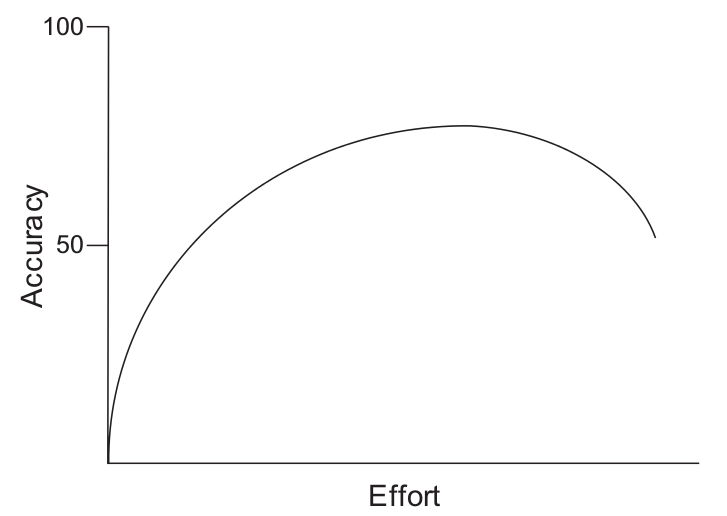
\includegraphics[scale=0.4]{figuras/effort_accuracy}
      \caption[Relação entre a acurácia e o esforço realizado para a estimativa.]
	      {Relação entre a acurácia e o esforço realizado para a estimativa. Fonte: \cite{cohn06}}
      \label{fig:effort_accuracy}
    \end{figure}
    
%Ideias para possíveis tópicos
% \section{Metodologia ágil}
% % 	\subsection{Estimativas em \textit{StoryPoints}}
% 	\subsection{Velocity}
% 	\subsection{Prazo de entrega
% 	\subsection{Atrasos na entrega}



